\chapter{Introduction}

Since the discovery of the Higgs boson~\cite{Aad_2012,Chatrchyan_2012,CMS:2013btf} at the LHC, an extensive program of measurements~\cite{PhysRevD.98.030001} has been undertaken to determine its properties and couplings to different types of particles and to assess whether these properties are consistent with those predicted by the SM. With the successful running of the LHC, large data samples of $\Pp\Pp$ collisions at $\sqrt s = 13\TeV$ have been accumulated, increasing the sensitivity to rare decays of the Higgs boson. 
Such decays also provide probes for possible contributions arising from BSM physics and include the process 
\hzg~\cite{Abba96, Chen12, Htollg-FB-Sun, Passarino, Campbell_2013hz, Degrassi:2019yix, Low:2011gn}.

Figure \ref{fig:fey} shows Feynman diagrams for the key SM contributions to the \hzg{} decay process. 
Experimentally, the final state resulting from $\PZ \to \ell^+ \ell^-$ ($\ell = \Pe$ or $\mu$) is the most accessible, since the leptons are highly distinctive, well-measured, and provide a means to trigger the recording of the events. 
\begin{figure*}[!b]
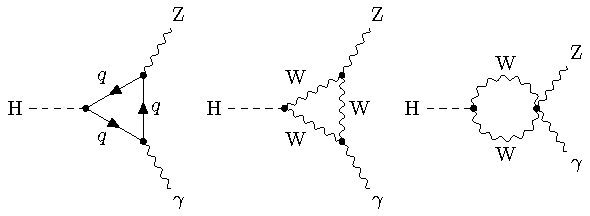
\includegraphics[width=0.9\textwidth]{fig/intro/Figure_001.pdf}
	\caption{Feynman diagrams for \hzg{} decay.} \label{fig:fey}
\end{figure*}
In the SM, the expected branching fraction for \hzg{} is $\mathcal{B}(\PH\to\PZ\gamma) = (1.57 \pm 0.09) \times 10^{-3}$, assuming a Higgs boson mass of $m_\PH = \mH\GeV$. This branching fraction is comparable to $\mathcal{B}(\PH\to\gamma\gamma)  = (2.27 \pm 0.04) \times 10^{-3}$~\cite{LHC-YR4,CMS:2021kom}. The value $m_\PH=\mH \pm 0.14\GeV$ is taken from the most recent CMS Higgs boson mass measurement~\cite{CMS:2020xrn}, which uses the combination of $\PH\to\gamma\gamma$ and $\PH\to\PZ\PZ^*\to 4\ell$ results from the $2011$--$2012$ and $2016$ data samples.
The ratio $\mathcal{B}(\PH\to\PZ\gamma)/\mathcal{B}(\PH\rightarrow\gamma\gamma) = 0.69 \pm 0.04$ is 
potentially sensitive to BSM physics, such as supersymmetry and extended Higgs 
sectors~\cite{Djouadi:1996yq,Zg_theory_extension,Zg_theory_decaywidth,Chen:2013vi}.
The effects from these models can shift the \hzg{} and $\PH\to\PGg\PGg$ branching fractions 
by different amounts, making the ratio the most sensitive observable. 
The impact on the ratio varies by model, but can be up to 20\% for two Higgs doublet or minimal supersymmetric models.

The ATLAS (A Toroidal LHC ApparatuS) and CMS Collaborations have performed
searches for the decay $\PH\to\PZ\gamma\to\ell^+\ell^-\gamma$~\cite{atl-HZG,cms-HZG,Sirunyan:2018tbk,Aad:2020plj} at $\sqrt{s}=7$,
$8$, and $13\TeV$ in the $\Pe^+\Pe^-\gamma$ and $\mu^+\mu^-\gamma$ final states. 
The most stringent bound has been set by the ATLAS Collaboration using $\sqrt s = 13\TeV$ data corresponding to an integrated luminosity of $139\fbinv$. The observed (expected) upper limit at 95\% confidence level (\CL) on $\sigma(\Pp\Pp\to\PH)\mathcal{B}(\PH\to\PZ\gamma)$ relative to the SM is $3.6$ ($2.6$), assuming $m_\PH=125.09\GeV$.
The ATLAS experiment has reported evidence at the 3.2 standard deviation level for the decay $\PH\to\ell^+\ell^-\gamma$ with $m_{\ell^+\ell^-} < 30\GeV$ using both of the dilepton channels~\cite{atlas_llgrun2}.
The CMS Collaboration has also searched for the
$\PH\to\ell^+\ell^-\gamma$ process with $m_{\ell^+\ell^-} < 50\GeV$\, in the dimuon channel at $\sqrt{s}=8$~\cite{2016341} and
$13$~\cite{Sirunyan:2018tbk}$\TeV$.  

This thesis describes a search for the decay $\PH\to \PZ\gamma$, where $\PZ\to\ell^+\ell^-$ and $m_{\ell^+\ell^-} > 50$ \GeV. 
This phase space is chosen in order to target on-shell Z bosons, since the region $m_{\ell^+\ell^-} < 50$ \GeV contains a contribution from an additional process, $\PH \to \gamma^* \gamma \to \ell^+ \ell^- \gamma$~\cite{Htollg-FB-Sun}.
The data sample corresponds to an integrated luminosity of \LumiT\fbinv of $\Pp\Pp$ collisions at $\sqrt s = 13 \TeV$ accumulated between 2016 and 2018. 
%The region at small dilepton invariant mass, $m_{\ell^+\ell^-} < 50$ \GeV, is excluded from the analysis. It contains a contribution from an additional process, $\PH \to \gamma^* \gamma \to \ell^+ \ell^- \gamma$~\cite{Htollg-FB-Sun}.
%The sensitivity of the analysis is enhanced by searching for Higgs boson production in a variety of mechanisms, including gluon-gluon fusion ($\Pg\Pg\PH$); vector boson fusion (VBF)
%; and the associated production of a Higgs boson with either weak vector bosons (V$\PH$, where V = $\PZ$ or $\PW$) or top quark pairs ($\ttbar\PH$). The dominant backgrounds arise from Drell--Yan production in association with an initial-state photon~($\PZ/\gamma^{*}$+$\gamma$) and Drell--Yan production in association with jets, where a jet or additional lepton is misidentified as a photon ($\PZ/\gamma^{*}$+jets). 
%After using a variety of discriminating variables to suppress background in the different production mechanisms, the signal is identified as a narrow resonant peak around $m_\PH$ in the distribution of the $\ell^+\ell^-\gamma$ invariant mass ($m_{\ell^{+}\ell^{-}\gamma}$).
%
%The data sample is divided into eight mutually exclusive categories according to (i) the presence of an additional lepton produced by $\PZ(\to\ell^+\ell^-)$ or $\PW(\to\ell\nu)$ decay, indicating the possible associated production of a Higgs boson with $\PW$ or $\PZ$ bosons, or $\ttbar\PH$ production with a leptonic top quark decay; (ii) the value of a multivariate analysis (MVA) discriminant characterizing the kinematic properties of a dijet system together with the $\ell^+\ell^-\gamma$ candidate, indicating possible VBF production; and (iii) the value of an MVA discriminant characterizing the kinematic properties of the $\ell^+\ell^-\gamma$ system. A simultaneous maximum likelihood fit is performed to the $m_{\ell^+\ell^-\gamma}$ distribution in each category. 
This thesis is organized as follows. The relevant theoretical physics background is provided in Chapter~\ref{sec:theory}, and the CMS detector and event reconstruction are described in Chapter~\ref{sec:experiment}. Chapter~\ref{sec:analysis_overview} provides an overview of the \hzg{} search strategy, and the data and simulated event samples are described in Chapter~\ref{sec:data}. Chapter~\ref{sec:selection} outlines the object and event selection, and Chapter~\ref{sec:categorization} discusses the event categorization using the MVA discriminants described above. The signal and background modeling procedure is presented in Chapter~\ref{sec:modeling}, with systematic uncertainties discussed in Chapter~\ref{sec:uncertainties}. Chapter~\ref{sec:statistics} describes the statistical procedure. The final results obtained from the fits are discussed in Chapter~\ref{sec:results}, followed by a conclusion in Chapter~\ref{sec:conclusion}.
